%%%%%%%%%%%%%%%%%%%%%%%%%%%%%%%%%%%%%%%%%%%%%%%%%%%%%%%%%%%%%%%%%%%%%%%%%%
%                                                                         %
%      This file is part of the 'openLilyLib' library.                    %
%                                ===========                              %
%                                                                         %
%              https://github.com/lilyglyphs/openLilyLib                  %
%                                                                         %
%  Copyright 2012-13 by Urs Liska, lilyglyphs@ursliska.de                 %
%                                                                         %
%  'openLilyLib' is free software: you can redistribute it and/or modify  %
%  it under the terms of the GNU General Public License as published by   %
%  the Free Software Foundation, either version 3 of the License, or      %
%  (at your option) any later version.                                    %
%                                                                         %
%  This program is distributed in the hope that it will be useful,        %
%  but WITHOUT ANY WARRANTY; without even the implied warranty of         %
%  MERCHANTABILITY or FITNESS FOR A PARTICULAR PURPOSE. See the           %
%  GNU General Public License for more details.                           %
%                                                                         %
%  You should have received a copy of the GNU General Public License      %
%  along with this program.  If not, see <http://www.gnu.org/licenses/>.  %
%                                                                         %
%%%%%%%%%%%%%%%%%%%%%%%%%%%%%%%%%%%%%%%%%%%%%%%%%%%%%%%%%%%%%%%%%%%%%%%%%%%

\documentclass[../../LilyPond-Tutorials]{subfiles}

\begin{document}
\parttitle[Urs Liska]{Arbeiten mit Textdateien für Musiker und Musikwissenschaftler}
\begin{authorAbstract}{Urs Liska}
Die meisten Musiker und Musikwissenschaftler bearbeiten Textdokumente und Partituren oder Notenbeispiele mit grafischen Programmen, ohne eine grundsätzliche Alternative überhaupt in Erwägung zu ziehen.
Der vorliegende Aufsatz zeigt demgegenüber einen Ansatz, der auf der Bearbeitung reiner Textdateien basiert.
Dieser Ansatz ermöglicht neuartige Wege gemeinschaftlichen Arbeitens, Forschens und Publizierens, indem jahrzehntelange Erfahrungen aus der Softwareentwicklung fruchtbar gemacht werden können.
Die beschriebenen Konzepte, Werkzeuge und Workflows haben mein Leben als Autor von Text- und Partiturdokumenten grundlegend verändert, und es ist mir ein großes Anliegen, sie der musikwissenschaftlichen Gemeinschaft zur Diskussion zu stellen.

\sloppy In den Geisteswissenschaften ist textbasiertes Arbeiten praktisch unbekannt, während es in vielen natur- und computerwissenschaftlichen Disziplinen zum Standard gehört.
Tatsächlich erfordert das Arbeiten mit Textdateien ein grundlegendes Umdenken, und es kann nicht geleugnet werden, dass dies mit einer nennenswerten Lernkurve verbunden ist.
Diese Investition erscheint mir jedoch mehr als gerechtfertigt, da sie auf lange Sicht die Produktivität ebenso erhöht wie die Qualität der Ergebnisse.

Der vorliegende Text ist eine stark verkürzte Fassung des englischen Originals, das unter \url{http://lilypondblog.org/2013/07/plain-text-files-in-music/} erhältlich ist.
Er verzichtet nach Möglichkeit auf ausführliche Erläuterungen (die im Original nachvollziehbar sind) und spitzt die Argumentation deutlicher auf die musikwissenschaftliche Perspektive zu.

Die wesentlichen Softwaresysteme, die ich auf den folgenden Seiten vorstellen -- in deren Benutzung ich aber nicht einführen -- werde, sind:

\begin{itemize*}
\item \emph{Versionsverwaltung} -- behält die Übersicht über Ihre Arbeit
\item \emph{LilyPond} -- das Notensatzprogramm
\item \emph{\LaTeX} -- das professionelle Textsatzsystem
\end{itemize*}

\end{authorAbstract}

\chapter{Textdateien als Grundlage}
\label{chap:pt_plain-text-format}
Im Gegensatz zu \textsc{wysiwig}-Programmen, die eine grafische Ansicht von Dokumenten bieten, ist bei der Bearbeitung von Textdateien das Ergebnis nicht unmittelbar ersichtlich -- der „Quelltext“ muss erst in ein grafisches Dateiformat „übersetzt“ oder „kompiliert“ werden.
Weshalb sollte man sich nun diese Abstraktionsebene aufbürden, wo es doch offensichtlich schnell, einfach und effizient ist, ein Dokument in seinem endgültigen Erscheinungsbild zu bearbeiten?
Ist es nicht nachgerade \emph{natürlich}, eine Partitur grafisch mit einer Maus zu bearbeiten?

Nun, es gibt eine Reihe guter Gründe, Dokumente als Textdateien zu speichern und zu bearbeiten.
Textbasiertes Arbeiten umgeht einige grundlegende Probleme anderer Ansätze, und es eröffnet Perspektiven auf ein breites Spektrum erweiterter Möglichkeiten.
Und schließlich gibt es heutzutage Bearbeitungsprogramme, welche den Umgang mit Textdateien erheblich vereinfachen.

Einleitend werde ich einige grundlegende Aspekte der Verwendung von Reintextformaten erläutern.

\section*{Transparenz und Kontrolle}
\label{sec:pt_transparency-and-control}
Grafische Programme (insbesondere solche mit proprietären Dateiformaten) lassen sich hinsichtlich der Speicherung und Interpretation eingegebener Inhalte i.\,d.\,R. nicht in die Karten sehen.
Einer der Hauptgründe, meinem grafischen Notationsprogramm den Rücken zu kehren, war dessen Angewohnheit, scheinbar willkürlich meine manuellen Änderungen zu überschreiben.

Etwas grundsätzlicher formuliert: Bei einem grafischen Programm habe ich keinen Einblick, 
\begin{inparaenum}[1)]
\item in welcher Form ein mit der Maus verschobenes Element gespeichert wird,
\item auf welche Referenz sich die Änderung bezieht und
\item wie das Programm meine Änderung bei einer Layoutanpassung (etwa auf Grund eines neuen Zeilenumbruchs oder Papierformats) behandeln wird.
\end{inparaenum}
Darüber hinaus ist insgesamt nicht ersichtlich, welche Elemente manuell angepasst wurden und welche dem automatischen Ergebnis entsprechen.

In einer Quelltextdatei hingegen ist unzweideutig definiert, welche manuellen Änderungen beabsichtigt sind, diese sind von Jedermann nachzulesen.
Und sollte einmal eine Änderung erhebliche Nebenwirkungen auf das Layout haben, so kann jede einzelne Modifikation gezielt verändert oder zurückgenommen werden -- während ich im grafischen Programm lediglich die Wahl habe, mein Glück mit einer \emph{Undo-}Funktion zu versuchen oder das Problem durch \emph{weitere} Korrekturen in den Griff zu bekommen.

Der Preis dafür ist die Notwendigkeit, den Quellcode händisch einzugeben und dies zunächst zu erlernen.
Doch lohnt sich der Aufwand auf lange Sicht.

\section*{Inhalt, Bedeutung und Erscheinungsbild}
\label{sec:pt_separation-content-meaning-appearance}
Die auf Grund der Allgegenwart grafischer Programme verbreitete Vorstellung, das \emph{visuelle Erscheinungsbild} eines Dokuments sei gleichbedeutend mit seinem \emph{Inhalt}, ist ein Trugschluss.
Tatsächlich handelt es sich dabei um zwei verschiedene Ebenen, die nur üblicherweise unter einer Benutzeroberfläche vereint sind.
Ein Text in einer Schriftgröße von 16\,Punkt etwa, der fett und kursiv dargestellt ist, kann auf verschiedenste Weise formatiert sein:
\begin{inparaenum}[1)]
\item als Absatzvorlage,
\item als Zeichenvorlage,
\item als manuelle Formatierung,
\item als Absatz- mit zusätzlicher Zeichenvorlage oder
\item als beliebige Mischung dieser Optionen.
\end{inparaenum}
Je nach Kontext können unterschiedliche Methoden adäquat sein, aus dem Erscheinungsbild einer grafischen Benutzeroberfläche wird jedoch die verwendete Formatierungsart nicht deutlich.

Im Quelldokument eines textbasierten Programms hingegen wird der Text explizit \emph{ausgezeichnet}.
Der Vorteil der strikten und sauberen Trennung zwischen dem Inhalt und dessen Erscheinungsbild überwiegt den Umstand, dass das Erfassen des Inhalts scheinbar schwieriger ist, wenn man bei einem Konstrukt wie „\texttt{Schuberts \textbackslash werktitel\{Winterreise\}}“ den Auszeichnungsbefehl mental ausblenden muss.

Im Falle von Partituren ist die Sache ähnlich gelagert:
Eine textbasierte Partitur-Eingabedatei enthält eine Repräsentation des musikalischen \emph{Inhalts}, während das \emph{Erscheinungsbild} erst während des Übersetzungsvorgangs entsteht und in der resultierenden \textsc{pdf}-Datei zur Verfügung steht.
Diese Kontrolle über die Trennung von Inhalt, Bedeutung und Erscheinung ist eine wichtige Grundlage für die Arbeitstechniken, auf die ich im weiteren Verlauf näher eingehen werde.

\section*{Lesbarkeit und Stabilität von Text- und Binärdateien}
\label{sec:pt_readability-stability}
Textdateien sind lesbar, Binärdateien nicht -- diese schlichte Feststellung hat grundlegende Implikationen für den Umgang mit digitalen Dokumenten.

Während die Eingabedatei eines (guten) Reintextformats präzise und lesbar den Inhalt des Dokuments beschreibt, enthält die proprietäre Binärdatei eines kommerziellen Programms einen unverständlichen Datenstrom, der nur von dem entsprechenden Programm oder einem geeigneten Importfilter eines anderen Programms interpretiert werden kann.
Inzwischen bieten zwar viele Programme (so auch \emph{Word} und \emph{OpenOffice}) die Möglichkeit, Dokumente in \textsc{xml}-Formaten abzuspeichern, die ebenfalls zur Gruppe der Textdateien gehören.
Das Verhältnis von tatsächlichem Inhalt und zusätzlichem \emph{Markup} ist dabei jedoch so ungünstig, dass diese praktisch nicht mehr lesbar sind%
\footnote{Im Anhang der englischen Fassung dieses Aufsatzes sind eine Reihe von Rohdateien einfacher Text- und Partiturdokumente abgedruckt, deren Studium an dieser Stelle nachdrücklich empfohlen wird.}.

Die Tatsache, dass Textdateien menschenlesbar sind, hat zwei wesentliche Implikationen:

\paragraph{Datenrettung}
Beschädigte Dateien können heutzutage auch dann \emph{teilweise} wiederhergestellt werden, wenn das Dateisystem zerstört wurde oder die Daten versehentlich gelöscht wurden.
Binärdateien jedoch, die nicht \emph{vollständig} rekonstruiert werden können, sind i.\,d.\,R. komplett verloren, selbst wenn nur ein Bruchteil der Datei beschädigt ist.

Bei der Wiederherstellung korrupter Textdateien hingegen kann praktisch alles, was rekonstruierbar ist, auch wiederverwendet werden, selbst, wenn man nur noch die bloßen Bytes der Datenträgeroberfläche abscannen konnte.
Mit etwas Glück lassen sich die fehlenden Puzzleteile leicht ergänzen.

\paragraph{Verwendung „antiker“ Dateien}
Mit der Weiterentwicklung von Software ändern sich deren Dateiformate.
Auch wenn Programme üblicherweise Dateien ihrer Vorgängerversionen öffnen können, wird deren Unterstützung irgendwann eingestellt, so dass zum Bearbeiten alter Dateien eine ältere Version des Programms erforderlich ist.
Bei einem Wechsel des Betriebssystems verschärft sich dieses Problem erheblich.
Daten werden in aller Regel irgendwann unbenutzbar.

Programme, die mit Textdateien arbeiten, unterliegen dieser Gesetzmäßigkeit ebenso, doch sind diese Dateiformate meist wesentlich besser dokumentiert, so dass die Wahrscheinlichkeit einer verfügbaren Konvertierungsmöglichkeit erheblich größer ist.
Und sollte alles nichts helfen, bleibt zumindest noch die „rohe“, menschenlesbare und frei zugängliche Datei, für die prinzipiell jederzeit ein neues Bearbeitungs- oder Konvertierungsprogramm geschrieben werden kann.

Textdatei-basierte Projekte können auf diese Weise -- insbesondere in Verbindung mit Versionskontrolle (siehe das nächste Kapitel) -- ungeahnte Zeiträume einer Vielzahl von Computergenerationen umspannen.
Dies macht diese Herangehensweise besonders geeignet für akademische Zwecke.

\section*{Editor-Unabhängigkeit}
\label{sec:pt_editor-independence}
Textbasierte Arbeitsumgebungen trennen das Bearbeiten, Verarbeiten und Anzeigen von Dokumenten.
Auf diese Weise ist man nicht an \emph{die eine} Anwendung gebunden, die vom (kommerziellen) Hersteller vorgegeben ist, sondern kann je nach Kontext beliebige Bearbeitungsprogramme verwenden.
Beispielsweise kann an einem Projekt gleichzeitig mit verschiedenen Werkzeugen gearbeitet werden, so können Skizzen ohne Weiteres auf dem Smartphone oder in einem Internetcafé notiert und später mit den Hauptdokumenten verbunden werden.
Ebenso ist das Textformat ein geeignetes Mittel, um Dokumente in einem Internetbrowser notieren zu können.
So gibt es inzwischen eine Reihe von Projekten, die aus Texteingabe im Browser Notation erzeugen können, am prominentesten die neue Wikipedia-Erweiterung%
\footnote{\url{http://en.wikipedia.org/wiki/Help:Score}}.

\section*{Programmierbarkeit}
\label{sec:pt_programmability}
Textdateien können nicht nur mit jedem Texteditor, sondern auch mit jeder Programmiersprache bearbeitet werden.
Die meisten Anwendungsprogramme bieten heute Schnittstellen für Skriptsprachen, mit deren Hilfe zusätzliche Funktionalität ergänzt werden kann.
Im Gegensatz zu diesen, vom Hersteller explizit vorgegebenen, Möglichkeiten können Textdateien jedoch in jeder nur erdenklichen Weise programmatisch bearbeitet werden: Man kann den Inhalt analysieren oder verändern, oder sie auch gänzlich neu generieren.
Die Liste möglicher Anwendungen ist lang und reicht (bei Partituren) von kontrapunktischen Operationen über algorithmische Komposition bis hin zur Verwaltung umfangreicher Beispielsammlungen in einer Datenbank (mit Internetzugriff).

Von dieser Option können auch Nutzer profitieren, die selbst nie programmiert haben und es auch nicht lernen wollen.
So kann in größeren Projekten mit Hilfe von Programmierung eine Infrastruktur geschaffen werden, welche die Komplexität vor dem Einzelnen gerade \emph{verbirgt}.

\section*{Unmittelbares Feedback vs. Übersetzung}
\label{sec:pt_compiling-instant}
Einer der Aspekte textbasierten Arbeitens, an den sich Benutzer am meisten gewöhnen müssen, ist das Fehlen eines unmittelbaren visuellen Feedbacks eingegebener Änderungen.
Grafische Programme reflektieren jegliche Änderung sofort, während die Eingabedatei des textbasierten Programms zunächst kompiliert werden muss.

Obwohl dies zunächst umständlich erscheint, ist es ein inhärenter bedeutender Vorteil.
Während der Arbeit im Dokumenteninhalt kann und \emph{muss} der Autor sich nicht mit Fragen des Layouts befassen, und das Programm muss nicht jede minimale Änderung sofort mit einem brauchbaren Ergebnis quittieren (was etwa bei einem größeren Textdokument mit vielen eingebetteten Abbildungen durchaus eine große Herausforderung ist und die Flüssigkeit des Arbeitens einschränken kann).
Dafür kann sich das Programm beim eigentlichen Übersetzungsvorgang genügend Zeit nehmen, um zunächst eine interne Repräsentation der \emph{Struktur} zu erzeugen und schließlich das Layout bestmöglich zu erstellen.

Die Konsequenz hieraus ist eine Standard-Ausgabe von erheblich höherer Qualität als bei grafischen Programmen%
\footnote{Für einige Beispiele siehe die englische Fassung des Aufsatzes}.
Als Faustregel kann man bei textbasierten Programmen (wie LilyPond und \LaTeX) davon ausgehen, sich erst dann mit Formatierungsdetails befassen zu müssen, wenn tatsächlich eine Veröffentlichung vorbereitet werden muss.
Dies ist auf lange Sicht ein erheblicher Vorteil, da man sich als Autor bis zur eigentlichen Druckvorbereitung auf den eigentlichen \emph{Inhalt} des Dokuments konzentrieren kann.

\bigskip
\hrule
\bigskip

Einige weitere Vorzüge der Arbeit mit Textdateien, insbesondere die Verwendung von \emph{Variablen}, kaskadierenden Set-ups durch \emph{Inklusion} von Dateien sowie die \emph{Kommentierung} und \emph{Dokumentation} von Quelldateien, werde ich im Kapitel \ref{chap:pt_lilypond} über LilyPond (ab S.\,\pageref{chap:pt_lilypond}) vorstellen.
Doch zunächst werde ich auf den vielleicht wichtigsten Aspekt textbasierten Arbeitens eingehen: \emph{Versionskontrolle}.

\chapter{Versionskontrolle}
\label{chap:pt_version-control}
Das Konzept der \emph{Versionskontrolle}%
\footnote{\url{http://de.wikipedia.org/wiki/Versionsverwaltung}}
ist vor allem aus der Softwareentwicklung bekannt, wo es bei Projekten ab einer gewissen Größe zum Standardrepertoire gehört.
Zu realisieren, dass es ebensogut für musikalische wie musikwissenschaftliche Zwecke nutzbar gemacht werden kann, war eine Erkenntnis, die meine Arbeitsmethoden grundlegend verändert hat.

In einer ersten Näherung kann man Versionskontrolle als eine unendlich flexible Ausprägung des \emph{Rückgängig/Wiederherstellen}-Mechanismus begreifen.
Versionierung dokumentiert die gesamte Entstehungsgeschichte eines Dokuments bzw. eines Verzeichnisses von Dokumenten und erlaubt es, \emph{jeden beliebigen} vergangenen Zustand des Projekts zu inspizieren oder wiederherzustellen.
Darüber hinaus erlaubt sie, jeden einzelnen Änderungsschritt individuell, d.\,h. nicht notwendig in chronologischer Reihenfolge zu widerrufen.
So kann etwa die Überarbeitung eines bestimmten Kapitels, die vor zwei Wochen durchgeführt wurde, rückgängig gemacht werden, ohne die sonstige seitherige Arbeit zu berühren.
Traditionellerweise wäre man auf das Vorhandensein eines Backups genau des gewünschten Zustands angewiesen und würde bei der Gelegenheit alle spätere Arbeit verlieren.

Es mag nicht selbsterklärend sein, aber dies kann ohne Weiteres Jahrzehnte, Programmwechsel und sogar Betriebssystemgenerationen überdauern -- weil Textdateien gewissermaßen zeitlos sind, wie im vorigen Kapitel erläutert wurde.
Die ältesten bekannten Software-Projekte, die heute noch entwickelt werden, haben eine kontinuierliche Versions-History seit den 80er Jahren des vergangenen Jahrhunderts.
Dies ist auch eine hervorragende Perspektive für (musikalische oder andere) Gesamtausgaben und vergleichbar langfristig angelegte akademische Projekte.

\section{Grundlagen der Versionskontrolle}
\label{sec:pt_basics-version-control}
Das Fundament der Versionskontrolle ist der zeilenweise%
\footnote{„Zeilenweise“ bezieht sich auf die Zeilen der Quelltextdatei.}
Vergleich eines gesamten Projektverzeichnisses.
Quelldatei-Zeilen beinhalten üblicherweise eine logische Einheit wie etwa einen Satz (in einem Textdokument) oder einen Takt einer Stimme in einer Partitur.
In einem sogenannten „Commit“ wird ein Satz zusammenhängender Zeilen-Änderungen in 
einem Projektverzeichnis zusammengefasst, es wird also eine Liste aller geänderten (z.\,B.) Sätze während eines Bearbeitungsschrittes dokumentiert.
Der Zuschnitt dieser Liste ist dabei frei wählbar:
Ein Commit kann die Korrektur eines Rechtschreibfehlers bzw. eines Taktstriches umfassen oder die Überarbeitung eines kompletten Kapitels.
Diese Menge von Änderungen wird -- mit einer erläuternden Beschreibung versehen -- der Projektgeschichte hinzugefügt und kann später zu jedem Zeitpunkt eingesehen, widerrufen oder verändert werden.

In diesem mächtigen zeilenweisen Ansatz liegt auch der Grund für die ausschließliche Anwendbarkeit von Versionskontrolle auf textbasierte Dateiformate.
In Binärdateien lassen sich Änderungen überhaupt nicht erfassen, und auch \textsc{xml}-basierte Formate eignen sich nur sehr bedingt für die Versionierung:
Allein durch das Öffnen und Speichern eines Dokuments (ohne tatsächliche Änderungen) werden so viele Zeilen der Datei verändert (etwa durch Angaben über Zeitstempel oder geöffnete Werkzeugleisten), dass der resultierende Commit praktisch nichtssagend wird.

Ein wichtiges und mächtiges Konzept der Versionskontrolle sind \emph{Zweige} (\emph{branches}).
Diese kann man etwa wie eine unabhängige „Sitzung“ verstehen, in deren Kontext man arbeitet, ohne die übrigen Sitzungen zu beeinflussen.
Ein üblicher und leicht verständlicher Verwendungszweck von Zweigen ist es, 
Arbeitsschritte abzugrenzen, die das Projekt zeitweise in einen inkonsistenten Zustand bringen.
So würde man beispielsweise die kritische Revision einer Notenausgabe im Rahmen eines Zweiges erledigen, wodurch die Partitur zu keinem Zeitpunkt eine Mischform zwischen Hauptquelle und revidierter Form aufweist.
Später lässt sich der Überarbeitungsvorgang dann jederzeit detailliert nachvollziehen.

\section{Gemeinschaftliches Arbeiten}
\label{sec:pt_collaborative-editing}

Der bedeutendste Aspekt jedoch, der akademischem Arbeiten wirklich neue Impulse verleihen kann, ist das von Versionskontrolle erheblich profitierende \emph{gemeinschaftliche Arbeiten%
\footnote{Der englische Begriff \emph{collaboration} erscheint mir dabei treffender.}}.
Dabei ist „Arbeiten“ in doppeltem Sinne gemeint: als Erarbeiten eines (Forschungs-)Gegenstands und als Bearbeiten von Dateien.
Versionskontrolle reduziert in erheblichem Maße Schwierigkeiten, die üblicherweise bei der gemeinsamen Bearbeitung von Dokumenten entstehen.

Die heute bei weitem verbreitetste Methode gemeinsamen Arbeitens besteht im Austausch von Dateien per Email, Datenträger oder der abwechselnden Bearbeitung im Netzwerk (oder der „Cloud“) lagernder Dateien.
Abhängig von der jeweiligen Einrichtung sind dabei mehr oder weniger umständliche Vorkehrungen erforderlich, um inkonsistente Datenzustände zu vermeiden.
Durch Austausch entstehende Kopien von Dokumenten müssen verwaltet werden, es muss dafür gesorgt werden, dass nicht zwei Personen gleichzeitig verschiedene Versionen des Dokuments verändern%
\footnote{Dies kann etwa geschehen, wenn ich ein vom Partner bearbeitetes Dokument zurückerhalte und weiterbearbeite, der Partner dann jedoch weitere Änderungen „nachreicht“},
und schließlich behindert das -- technisch oder durch Vereinbarung bedingte -- „Sperren“ von Dokumenten das freie Arbeiten.
Und schließlich wird eine derart gestaltete Zusammenarbeit vollends unpraktikabel, wenn dabei eine große Zahl von Dokumenten von mehr als zwei Mitarbeitern benutzt werden soll.

Hier nun setzt Versionskontrolle an.
Die Verwendung von Textdateien in Verbindung mit Versionskontrolle ermöglicht es, von jahrzentelanger Erfahrung in der Softwareentwicklung zu profitieren.
Deren Techniken und Strategien wurden insbesondere entwickelt, um die reibungslose Zusammenarbeit zahlreicher Mitarbeiter zu gewährleisten%
\footnote{So zählt beispielsweise das Linux Kernel Projekt mehrere Hunderttausend Commits von über zehntausend Beitragenden (es gibt leider keine adäquate Übersetzung für das passendere \emph{contributor}).}.

Der Kern einer gemeinschaftlichen Arbeitsumgebung ist eine gemeinsame Datenbasis, ein auf einem Server gespeichertes \emph{repository}, das allen Mitarbeitern zugänglich ist (wobei auch gestaffelte Rechte vergeben werden können).
Jeder Mitwirkende verfügt über eine lokale Kopie des Datenbestands, in der er uneingeschränkt arbeiten kann, auch ohne permanent mit dem Server verbunden zu sein.
Bei Gelegenheit gleicht er den lokalen und den zentralen Datenbestand miteinander ab, kann gezielt Beiträge anderer Mitarbeiter inspizieren und schließlich seine eigene Arbeit in den gemeinsamen Datenbestand integrieren.

Die beschriebene zeilenweise Vorgehensweise der Versionsverwaltung spielt nun ihre Vorteile bei verteiltem Arbeiten vollends aus, indem sie jegliches Sperren von Dateien überflüssig macht.
Und es kann nicht genug betont werden, dass das \emph{gleichzeitige} Bearbeiten von Dateien grundsätzlich kein Problem darstellt:
So könnte beispielsweise ein Herausgeber Fingersätze bearbeiten, während ein anderer die kritische Revision durchführt.
Solange die beiden nicht \emph{dieselbe Quelltextzeile} verändern, wird die Versionskontrolle alles transparent und unbemerkt integrieren.
Dies zielt nicht darauf ab, Konflikte \emph{unwahrscheinlich} zu machen -- das wäre fahrlässig.
Sollte das System Dateiversionen nicht selbständig zusammenführen können, wird der Bearbeiter auf die divergierenden Zeilen hingewiesen und kann den Konflikt manuell auflösen.
Versionierung kann und wird also Bearbeitungskonflikte nicht verhindern, garantiert jedoch, dass sie mit minimalem Aufwand behoben werden können, und zwar ziemlich unabhängig von der Anzahl der Mitarbeiter und betroffenen Dateien.

\medskip
Ein weiterer wichtiger Aspekt ist die Art und Weise, wie Änderungen am Datenbestand dokumentiert werden.
Wie beschrieben speichert ein \emph{commit} einen Satz an Änderungen, der später eingesehen werden kann.
Möchte ich also Änderungen beurteilen, die ein Partner eingebracht hat, so werden mir diese direkt angezeigt, ohne dass ich in den Dokumenten nach ihnen suchen müsste.
Im Gegensatz zu entsprechenden Funktionen, die zum Beispiel Textverarbeitungen bieten, ist diese Dokumentation permanent und verschwindet nicht, nachdem die Änderungen akzeptiert oder verworfen wurden.
Und bei Partituren wüsste ich nicht, wie ich außer mit einem -- fehleranfälligen -- AB-Vergleich den Korrekturdurchgang eines Anderen in einem grafischen Notationsprogramm überhaupt überprüfen könnte.


\medskip
Zusammenfassend kann man sagen, dass in einem Projekt unter Versionskontrolle eine beliebige Anzahl von Mitarbeitern auf einen beliebig großen gemeinsamen Datenbestand zugreifen kann.
Versionskontrolle garantiert die Minimierung von Zusammenführungskonflikten, bietet einfache Mittel, diese im Fall des Falles aufzulösen und verwaltet die Projekt-History sauber und transparent, notfalls auch über Jahrzehnte.
Dies eröffnet vielversprechende Perspektiven für akademische Projekte und Arbeitsweisen, von denen ich im abschließenden Kapitel ab S.\,\pageref{chap:pt_applications} einige näher vorstellen werde.

\chapter{LilyPond}
\label{chap:pt_lilypond}
When it comes to engraving musical scores my tool of choice is \emph{GNU LilyPond}%
\footnote{\url{http://www.lilypond.org}}.
Not only do I love its beautiful score output, but I really value how seamlessly and professionally I can integrate scores with (\LaTeX) text documents, and I have come to absolutely rely on the workflows and concepts based on the plain text approach that it allows.

Of course I would love to give you a thorough introduction to this amazing software but that would be quite pretentious and especially out of scope of this article.
Therefore I will keep my focus on the potentials of the text based approach, giving you just enough information to get an impression on how it would “feel” to work with it and to get the necessary foundation for the following ideas.

As you know quite well by now LilyPond works by reading in text files and processing them to engraved scores.
So one effectively \emph{has} to learn how music is represented in LilyPond's input language.
But it may be good to know that while it is actually possible to edit the text files with any plain text editor there actually \emph{are} graphical programs assisting you heavily in dealing with the text files.
Although there are a few I will only show you one.

\section{Frescobaldi}
\label{sec:pt_frescobaldi}

\textit{Frescobaldi%
\footnote{\url{http://www.frescobaldi.org}}}
is a complete editing environment that allows you to do everything you need within one interface.
In that it is quite similar to the graphical programs I have earlier dismissed as conceptually flawed.
But there is a big difference, as Frescobaldi presumably offers the best of both worlds:
it gives you the greatest possible graphical access to the editing process while in its core still being a---sophisticated---text editor.

Its main window presents itself like many programs that allow to edit textual source files of graphical documents: it is split in a \emph{text editor} and a \emph{music view} (see \fref{fig:pt_fb-main-window}).
In the music view on the right hand you see (surprise) the music.
Please note that a) Frescobaldi isn't responsible for generating the engraving in this view and b) this view doesn't have a  “live“ connection to the source but is only updated when LilyPond is run.
So you could actually call Frescobaldi a \textsc{wysiwyg} editor because what you see actually \emph{is} what you finally get---but you can't (yet) edit the score in a graphical way in this music view.
On the left side of the screen shot you can see the \emph{Quick Insert} widget, one of the tools that simplify your life by “remembering” how to insert all sorts of graphical symbols for you---but again: they won't insert them “into the score” but as text into your input file.

\begin{figure}
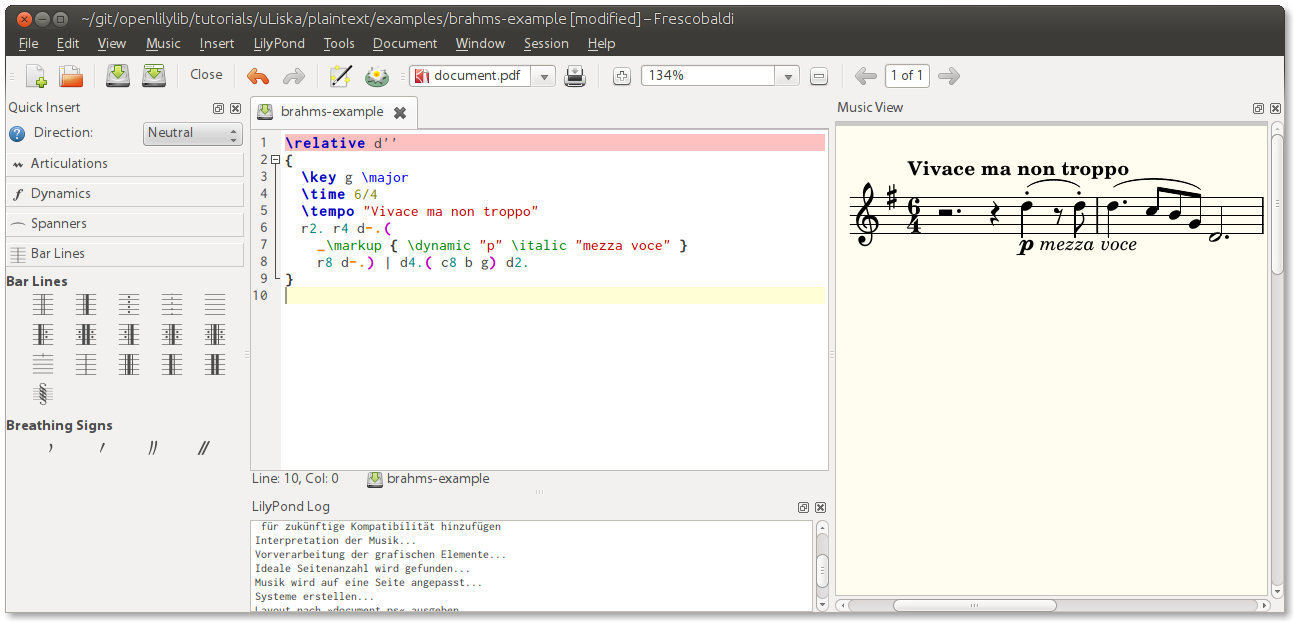
\includegraphics[max width=\textwidth]{examples/frescobaldi/main-window}
\caption{Frescobaldi's Main Window}
\label{fig:pt_fb-main-window}
\end{figure}

Another example of the useful tools is the \emph{Score Setup Wizard} that allows you to graphically configure a score of arbitrary complexity (just like in other programs) and that generates the text used for the corresponding score for you (see \fref{fig:pt_fb-score-setup-wizard}).

\begin{figure}
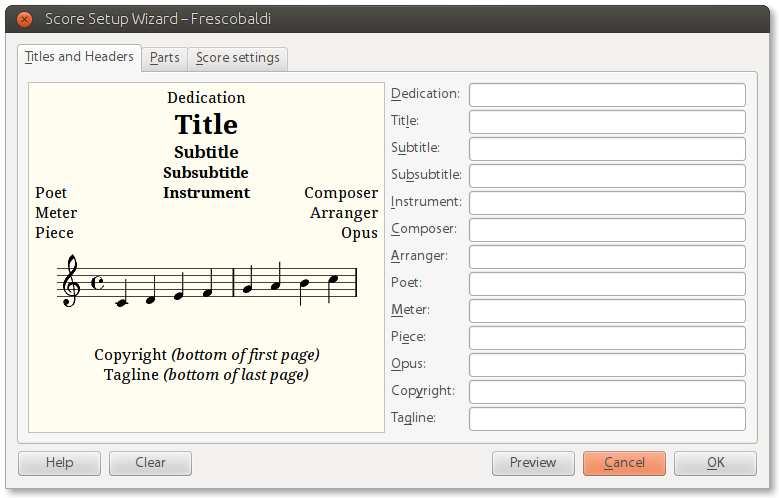
\includegraphics[max width=\textwidth]{examples/frescobaldi/score-wizard}
\caption{Frescobaldi: Score Setup Wizard}
\label{fig:pt_fb-score-setup-wizard}
\end{figure}

If you look at the text editor again (in \fref{fig:pt_fb-main-window}) you will see that the text is colored a lot (I will talk about the actual text soon).
This is a feature that Frescobaldi shares with most programming editors: it “knows” LilyPond's language and highlights the source text according to its structure.
Once one has got used to that practice it greatly eases reading and writing the necessary text files.

When you start typing a command Frescobaldi can also make suggestions on how to complete them (\fref{fig:pt_fb-code-completion})---also a valuable assistance, not so much because of its time-saving but because it assists your memory and efficiently reduces errors.

\begin{figure}
\centering
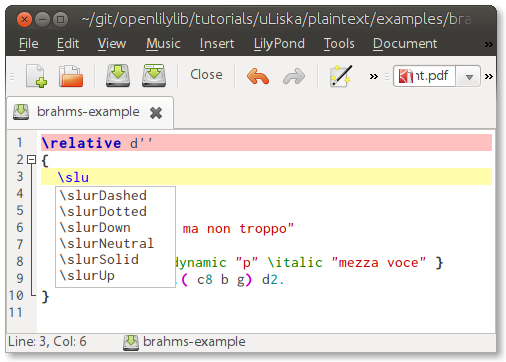
\includegraphics[width=8cm]{examples/frescobaldi/code-completion}
\caption{Frescobaldi: Suggestions for available commands}
\label{fig:pt_fb-code-completion}
\end{figure}

But maybe the most important feature for daily work is that you can click on an element in the music view and will be taken to the corresponding place in the input file.
In \fref{fig:pt_fb-point-and-click} you can see the slur highlighted in purple in the music view and the highlighted text in line 8 in the text editor.
\begin{figure}
\centering
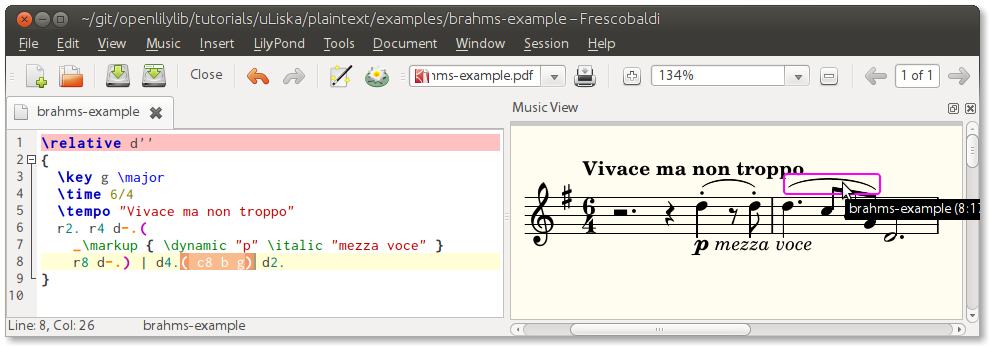
\includegraphics[max width=\textwidth]{examples/frescobaldi/point-and-click}
\caption{Frescobaldi: Two-way link between input file and score}
\label{fig:pt_fb-point-and-click}
\end{figure}
This also works in the other direction: If you select text in the editor the corresponding notation elements are highlighted in the score.
This lets you easily navigate your text file(s) and removes a handicap one could have seen in editing plain text files in the past.

One focus of current Frescobaldi development is the enhancement of the music view's functionality.
So it will soon be possible to partially “edit” the score with the mouse---of course in fact you will be able to tweak something visually and Frescobaldi will insert the appropriate text in the source file, possibly giving you the option to select from different approaches.
Currently there are plans to implement (e.\,g.) correcting pitches, drawing and shaping curves, and annotating objects (see also \fref{sec:pt_lilypond-comments}).
This will make “working with text files” even more comfortable.

Of course these remarks were only a very cursory overview of Frescobaldi.
A thorough introduction can't be the intention of this paper, but I wanted to give you a feeling to what extent current and smart editors can smoothen your editing experience.
Now you are ready to learn something about how LilyPond input files actually work.

\section{Textual Representation of Music}
\label{sec:pt_textual-representation}
In \fref{fig:pt_fb-main-window} (and \fref{fig:pt_fb-point-and-click}) you have seen a short score excerpt from Brahms' first violin sonata, along with the LilyPond code that produced it.
Now I'll use that example to show you a little bit about the basic elements in a LilyPond score.

At the most basic level notes are represented by their pitch and duration, as you can see in this “bare” example:

\begin{multicols}{2}
\begin{Verbatim}[samepage=true,
				   commandchars=|„“]
{
  r2. r4 d r8 d
  d4. c8 b g d2.
}
\end{Verbatim}
\columnbreak
\lilypondSFE{examples/brahms/brahms-1}
\end{multicols}

The text writes rests (\texttt{r}) and pitches (\texttt{d} etc.) as well as durations (8, 4, 4., 2.), and everything is enclosed in a pair of curly braces.
This is LilyPond's notion of a \emph{music expression}.
A score is represented by one big music expression which can be constructed of (or split into) arbitrarily nested or chained smaller music expressions.
There are a few things “missing” in the source that LilyPond adds by itself, namely a staff, a clef, and beams.

Two more elements aren't actually figured out automatically, but hidden from the example.
In fact you have to write down \cmd{key g} \cmd{major} and \cmd{time 6/4 }to tell LilyPond about the key and time signatures.
But the beaming in the second measure is done automatically according to the time signature.
Many things can be defined by such \emph{commands}.

Elements like articulations or dynamics are attached to notes or rests by printing them after the reference item, like in this fake example:

\newcommand{\hilite}[1]{\textcolor{red}{\textbf{#1}}}

\begin{multicols}{2}
\begin{Verbatim}[samepage=true,
				   commandchars=|„“]
{
  r2. r4 d|hilite„-.“ r8 d|hilite„-.“ 
  d4.|hilite„\sf“ c8|hilite„\>“ b g|hilite„\!“ d2.|hilite„->“
}
\end{Verbatim}
\columnbreak
\lilypondSFE{examples/brahms/brahms-2}
\end{multicols}

We have a few articulations that are attached with a hyphen, the staccato dot written as a dot, the accent as a \texttt{>}, all characters have been chosen to be as intuitive as possible.
Dynamics are attached by a backslash, in the example we have the \lilyDynamics{sf} with \cmd{sf}, the \decrescHairpin with \cmd{>}, and (as the only unusual item) the \cmd{!} which represents the \emph{end} of the hairpin.

We can attach \emph{spanners} to pairs of notes, e.\,g.\ the slurs in the following example.
Slurs are written as opening and closing round brackets (\emph{after} the note they are referring to)
There you can see that you can attach multiple items to a note by just writing them one after another

\begin{multicols}{2}
\begin{Verbatim}[samepage=true,
				   commandchars=|„“]
{
  r2. r4 d-.|hilite„(“ r8 d-.|hilite„)“
  d4.|hilite„(“ c8|hilite„[“ b|hilite„]“ g|hilite„)“ d2.
}
\end{Verbatim}
\columnbreak
\lilypondSFE{examples/brahms/brahms-3}
\end{multicols}

In addition to the slurs you can also see an example of manually setting the beams against the rules for the time signature, which is indicated by the use of square brackets (again \emph{after} the notes they are referring to).

In the last example of this \emph{very} short introduction to LilyPond files we'll add the necessary text elements to the score.
The \emph{tempo} indication is entered by the \cmd{tempo} command (the non-verbal part is here as an example only), while the \lilyDynamics{p} \emph{mezza voce} is a \cmd{markup}---a text that is attached to a note like any articulation or dynamic sign.

\begin{multicols}{2}
\begin{Verbatim}[samepage=true,
				   commandchars=|„“]
{
  |hilite„\tempo“ "Vivace ma non troppo" |hilite„2. = 60“
  r2. r4 d-.(|hilite„-\markup“
    { \dynamic "p" \italic "mezza voce" } 
    r8 d-.) 
  d4.( c8 b g) d2.
}
\end{Verbatim}
\columnbreak
\vspace*{4.5em}
\lilypondSFE{examples/brahms/brahms-4}
\end{multicols}

One thing you may have noticed in this last example is that I have broken the first line of music into three.
LilyPond doesn't care about this \emph{white space} and allows you to lay out your text file as you find appropriate---which usually will mean to keep coherent entities on a single line so that versioning will work optimally.
In this case the entity is the \emph{markup}, also an expression enclosed in curly braces.
You could just throw some text in there, but in this score we format the elements, one using the dynamics font, the other as italic text.

\medskip
Now you've seen your first real-world example of a LilyPond score.
Of course the complexity of these text files increases when the music gets longer or more complex.
But when looking at an input file you should always keep in mind that it is built from very small and rather simple units.
And you should feel comfortable with knowing that there are editors at hand that really help you navigating and editing them.

\section{Variables and Includes}
\label{sec:pt_variables-includes}
In the previous section I wrote that LilyPond adds necessary elements to what you have entered.
In the case of a file just consisting of a music expression as in our example it will actually add the necessary context for a staff, the score, and a “book” which represents the output file.
This works only for simple scores such as music examples or maybe plain chants, but for most real scores you will have to define the score structure explicitely.
While one would perhaps start with writing the music expressions directly inside the score set-up, there is the concept of \emph{variables} that proves infinitely useful for any project of some dimensions.

The basic structure of a score looks like this:
\begin{quote}
\begin{verbatim}
\score {
  \new Staff { ... music expression ... }
  \layout{}
  \midi{}
}
\end{verbatim}
\end{quote}

Inside the score block there is one \emph{Staff} that contains a music expression (I could have pasted the code from the previous examples here). \cmd{layout\{\}} tells LilyPond to create a score, the optional \cmd{midi\{\}} block additionally creates a \textsc{midi} file.
Instead of just \cmd{new Staff} there would be the complete structure of all (potentially nested) staves of the score, so the file would soon become very complex and confusing.
To avoid this one wraps up the music definition in a variable (e.\,g.\ \texttt{violin = \{ ... music ... \}}) and simply writes \verb+\new Staff \violin+ in the score block.

\medskip
Reading this you might consider it just a detail of the input file structure and wonder how this relates to you.
But packaging musical expressions in variables isn't only useful to reduce the complexity of the score block but serves many more goals.
It is a way for transparently and robustly store, use \emph{and reuse} blocks of music.
Reusing music is very useful, not only for the---admittedly quite specific---case of musical snippets or patterns, but also for the fundamental handling of the needs of musical engraving.
Earlier I wrote about the separation of content and appearance, here we are dealing with separation of the \emph{definition} and \emph{use} of music.
Music defined in a variable is used by a score---and it can equally be used by another score.
Different scores accessing shared music may be a full score and the instrumental parts or different transpositions of the same song.
In both cases the music is defined only once, and any update to that definition is propagated to all scores automatically.
This makes the handling of scores and parts very robust in LilyPond.

Being able to reuse variables would only be a partial advantage if one couldn't separate the definitions even one step further, into separate files, and \emph{include} them.
This way one can create a collection of files, a \emph{library}, and keep them available for further use.
This is not only useful for reusing work in future projects but also within one project.
You can organize style and layout templates (i.\,e.\ definitions that influence the page layout and the appearance of the music) in a hierarchical and sophisticated way and have all files share some common styles (like font selections) but have different additional styles for different output formats (full score, part, music example \dots).
Any change in one of the style files is then automatically propagated to all scores.
Or you can make use of a technique called \emph{commenting out}---place two alternative includes but comment one of them out, like this:

\begin{Verbatim}
\include "draft-layout.ily"
%\include "publish-layout.ily"
\end{Verbatim}

The second line of this is a \emph{comment}, so only the draft-layout file will be included (and may color editorial additions red, print additional information about the date or whatever you like to define) as long as you are working on the score.
When you're finished and prepare the final printout you can just move the percent sign one line up and get your final publication layout.
And if you have this construction in a shared style file this switch will have global affect to all scores that are part of your project.

\section{Comments}
\label{sec:pt_lilypond-comments}
The last example of the previous section led us smoothly to the next aspect: \emph{comments}.
LilyPond---as virtually all plain text formats---allows you to mark parts of a file as comments, i.\,e.\ text that will be ignored by the typesetting.
This can for example be used to comment on technical issues you are facing.
You could for example explain why you have decided to implement a certain voice-leading to solve a typographic problem, or leave a mark that some issues will have to be resolved.
Combine this with the fact that all your manual interventions are written explicitely in the file and compare that with the situation of a graphical score editing program where you can hardly even tell what your manual interventions were \dots

Currently there are plans to greatly enhance this functionality, especially with preparing scholarly editions in mind.
It will be possible to enter specific comments in the input file---\emph{i.\,e.\ directly beside the music they are referring to}---and a tool that will be called \texttt{lilypond-doc} will output them to a variety of formats.
This will provide nicely formatted lists of 
\begin{inparaenum}
\item \textsc{todo} items,
\item musicological questions,
\item typographical questions, and finally
\item critical remarks.
\end{inparaenum}
The items in the list will be smartly linked, so that clicking on them will point you directly to the corresponding place in the source file.
\emph{Frescobaldi} will probably be able to allow you to insert such comments directly from within the music view, so you can click on a note and enter the comment.
This way you will be able to do all your work \emph{within the actual score} (and collectively with your collaborators), and finally you will get the entries for the critical report nicely sorted and formatted as source text to be used in the corresponding \LaTeX{} document!

\section{Conclusion}
\label{sec:pt_lilypond-conclusion}
By now it surely won't make you wonder that I wholeheartedly endorse the use of LilyPond as a notation software.
I can't recommend highly enough to give it at least a try---but you should give it a fair try and expect some time and effort needed initially.
From my experience (having once been a beginner myself and from seeing other beginners) I may give you some advice on \emph{dos} and \emph{don'ts}:

Do \emph{not} jump right in and try to accomplish a complex project that has to be finished in time, or you will surely run into frustrations.
Ideally you should first read and follow the „Learning Manual“%
\footnote{\url{http://www.lilypond.org/doc/v2.16/Documentation/learning/index.html}}
from LilyPond's excellent documentation which will introduce you smoothly to the basic concepts.
But you may also tackle a task that is „real“ and on your desktop already.
This will make it more interesting, but be sure that it isn't too complex and that you won't have to struggle with deadlines.

Be sure \emph{not} to try it completely on your own, alone with you and the documentation.
The ideal way would be to have someone mentoring you, giving you the right ideas and giving the right answers to the questions that really matter at a time.
Of course this isn't available for most of the beginners, so be sure to sign up to the \texttt{lilypond-user} mailing list%
\footnote{\url{https://lists.gnu.org/mailman/listinfo/lilypond-user}}.
Reading the discussion there (and skipping what seems too complicated for now) will be helpful to get a feeling for it, and the community is usually very responsive and helpful, as long as you show interest and own efforts.

Be sure to get used to using the documentation.
As mentioned it is excellent, but apart from the Learning Manual it is a \emph{reference} that mostly won't guide you through the concepts.
You will have to read things more than once, and for the starting time you will need to lookup things quite often.
Even later you will need to have good access to that reference.
So you should make yourself acquainted with the layout of the documentation as soon as possible.

\medskip
Admittedly it takes some time and effort to get productive with LilyPond.
But the benefits clearly outweigh that in my opinion.
First of all you instantly get beautiful output that is pleasing the eye.
LilyPond's very existence is due to the frustration two musicians had with the anemic sheet music they were confronted day to day on their orchestral music stands.
Therefore LilyPond's first ideal and models are traditional, hand-engraved scores, and you (and your readers) will benefit from that saturated page impression out-of-the-box and in each score.
Practically this means that you will have \emph{significantly less work} to tune a score to be usable as performance material than when creating it with the known graphical programs (or the other way round: If you don't do that work at all (as obviously many composers do) the resulting material will be vastly superior).
If you want to prepare scores for publication you will probably have to spend time with LilyPond too, applying a smaller number of corrections which will each  take more time than with the graphical programs.
But as explained these corrections are much more robust, can be tracked and modified with a clean interface.

The other aspect of output quality is at least as important:
Since you get \emph{usable} results by default you can concentrate on the content much longer and only care about engraving details when actually preparing the final printout for publication.
But \emph{if} you want to apply manual modifications while still working on the content you have them in a clean and traceable way, and they won't step in the way when the final beautification takes place.

But what really sets working with LilyPond apart is the potential of new workflows powered by the plain text approach, as I have described in the previous chapters.
Seamlessly integrating work with others through versioning, documenting your work \emph{in situ}, setting up sophisticated and cascading style sheets on „house“, project or file level are the keywords to be mentioned here.
Interfacing scores or examples with \LaTeX{} documents will be one more topic, to be discussed in the next chapter.

\medskip
It wouldn't be honest to conceal one issue that I haven't touched so far: LilyPond's behaviour towards exchanging documents with other software.
Currently using LilyPond is kind of a one-way street with the only exit being the score in one of the various graphical output formats.
There are several ways to export/convert documents from other programs to be engraved by LilyPond (although you should expect some manual work to be done), but you can't simply export LilyPond input files to formats that can be used by other programs.
This usually isn't an issue when you are just creating scores to be printed, such as performance or teaching material, or music examples for books.
But it can be a show-stopper if you are preparing editions for commercial publishing houses because the majority of them has their established workflows and insists on getting the scores delivered as Finale\texttrademark{} or Sibelius\texttrademark{} files.
As you surely can imagine by now I wouldn't ever want to miss the plain text approach in preparing editions, so I would prefer doing it that way even if I knew (and felt sorry about it) that the score would end up being printed by one of the two programs.
So at least for this application it is a big desideratum to get LilyPond to export to MusicXML, a common interchange format.
As it stands, it doesn't even seem to be a major rewrite of the program but rather a few months of programmer's work.
Maybe \emph{one} rather large project with a sufficiently large organisation capable of bringing up some money would be enough to fix the situation.
But unfortunately there can't be any promises when (and if at all) this hole will be closed.

\chapter{\LaTeX}
\label{chap:pt_latex}

\LaTeX{} is for typesetting text documents what LilyPond is for typesetting scores.
It provides typesetting as opposed to mere text processing, providing the usual document author---who doesn't know too much about the rules of typography---with the necessary expertise to produce professionally typeset documents.
And it works by compiling plain text input files, so everything I have written about the advantages of using plain text files applies to \LaTeX{} equally.
Therefore I won't get into details introducing you to the concrete syntax of its input files, but try to introduce you concisely to some of the specifically musical features.

Your interface to \LaTeX{} is the same as to LilyPond:
The input files can be edited with \emph{any} editor, and the compilers are command line programs.
But there are (quite numerous) dedictaed editors or IDEs%
\footnote{Integrated Development Environments}
that assist you in editing the documents and organizing the compilation process for you.
Earlier in \fref{sec:pt_separation-content-meaning-appearance} I showed you a basic \LaTeX{} document in which you saw the three fundamental elements: the \emph{document class}, \emph{commands} and \emph{environments} (although I didn't explicitely name the latter).
As mentioned the document class is somewhat comparable to a document template in an office application.
But it is much more powerful in that it can contain many layout elments, commands and more functionality.
The LaTeX{} distribution contains many document classes for many purposes (from standard articles over beamer presentations to classes specific to fields of research), but you can also download classes from other sources, and you can (and will) write your own.
One important aspect of document classes is the selection of \emph{packages} to be included.

When run on a basic document as in our example \LaTeX{} only loads a small subset of its possibilities in order to save time and memory.
If you need additional functionality you can include it through the use of \emph{packages}.
Such a package might contain anything from a small set of related semantic markup commands up to sophisticated bibliographic functionality%
\footnote{See \url{http://en.wikibooks.org/wiki/LaTeX/Package_Reference} for a list of some packages with short comments on their functionality}.
When you want a different style for tables or lists, to include images, or add music examples---chances are good that there is a package enabling just what you need.

As I have also mentioned earlier the \emph{commands} and \emph{environments} are roughly similar to character and paragraph styles as used in office documents.
But they too are much more powerful because they are more like programmer's commands, especially as they can use arguments.
A command can do anything with its arguments which makes it a very versatile tool.
As a single example I have a command for entries in a revision report that takes arguments for measure number, position in the measure, affected voice/system, and the actual comment.
This information it then processed to a nice layout, skipping the separator characters when an argument is empty.
If I should decide upon a completely different layout I just have to update the command to propagate it to the whole document---or a complete set of documents if I have defined it in a package.
And of course I will soon be able to incorporate the report entries that \texttt{lilypond-doc} will give me from within the LilyPond scores \dots

\emph{Environments} are somewhat similar, with the difference that the commands are a one-time event while environments have a begin and an end (like the \emph{document environment} seen in the initial example).
Environments like \env{figure} or \env{table} allow you to place graphical items as \emph{floating} objects.
This allows \LaTeX{} to place them at the best position concerning the page breaking.
While this is something one has to get used to it is actually a big enhancement towards a \emph{professional} typesetting, especially of books and similar documents.
As producing books is the basic motivation for \LaTeX{} you also can expect professional tools with regard to bibliography, indices or figure lists etc.

\medskip
Now that we have seen a \emph{very} short introduction to \LaTeX{} it is time to consider some specifically \emph{musical} aspects to authoring text documents.

\section{Music Examples}
\label{sec:pt_music-examples}
Of course you can embed images in text documents if you want to add music examples to a text.
\LaTeX{} does a very good job at determining the best possible layout for them.
But there are a few dedicated tools that aid you with this specific task, in particular I will talk about \package{lilypond-book} and \package{musicexamples}.

\subsection{lilypond-book}
\label{subsec:pt_lilypond-book}
The program \package{lilypond-book} is part of the LilyPond distribution and allows to embed LilyPond source code directly in \LaTeX{} documents.
First you run \package{lilypond-book} on the document, which will call LilyPond to generate all (necessary) examples and create a copy of the document including these generated files.
Then you run \LaTeX{} to compile this processed copy.
This procedure has some overhead due to the large number of intermediate files, and many people using \package{lilypond-book} with complex documents or on a regular basis actually approach this using self-made scripts.
But if you have documents with lots of (small) examples you won't find any better solution to manage your music sources \emph{in situ}.

\subsection{musicexamples}
\label{subsec:pt_musicexamples}
Another way to embed music examples in \LaTeX{} documents is \package{musicexamples}, a package that is part of \openlilylib%
\footnote{\url{http://www.openlilylib.org/musicexamples}}.
Originally started as an alternative approach to \package{lilypond-book} not requiring intermediate documents it can actually work together with it quite well.
\package{musicexamples} provides environments and commands to include and manage music examples in \LaTeX{} documents.
There is support for floating and non-floating environments, single-line or multi-line examples (with the multi-line ones being able to be split on several pages).
You can also print full-page examples, with special support for examples starting on odd or even pages (you can force an example to start at the next odd or even page).
All examples in a document share the same counter and can be exported to a contigious list of music examples.

It is possible to use \emph{any} images for your music examples, but there is special support for using LilyPond (of course).
There are tools compiling your LilyPond files to files that can directly be used in the \LaTeX{} document, especially taking care of the odd/even issue.
This may be the way for you if you want to manage your scores separately from the text document.
Finally there will be%
\footnote{This part of the package hasn't been implemented yet.}
helper scripts that keep the music examples up to date (and conditionally recompile missing music example files).

Instead of existing image files (LilyPond generated or not) you can equally embed LilyPond code with \package{lilypond-book} and benefit from both approaches:
\package{lilypond-book}s in-place example code and \package{musicexamples}' example management.

You can see a comprehensive example document with all sorts of music examples in \fref{xmp:musicexamples-document}.

\subsection{OOoLilyPond}
\label{subsubsec:pt_ooo-lilypond}
Finally I have to mention another option to integrate music examples in text documents, although it isn't quite as professional.
\emph{OOoLilyPond}%
\footnote{\url{http://ooolilypond.sourceforge.net/}}
is an OpenOffice extension which allows to store LilyPond code as embedded objects in Writer documents.
It can compile them in place and display the corresponding image files while keeping the source code ready for further editing.
Unfortunately this can only produce bitmaps and no vector graphics, resulting in a rather medium output quality. But for daily use it may be a good compromise.

\section{Notational Elements}
\label{sec:pt_notational-elements}
Another member of our family of resources is \lilyglyphs[scale=1.1].
This package allows to include LilyPond's notational elements in the continuous text of \LaTeX{} documents.
This is significantly different from entering music examples as it will embed them as characters, like \lilyDynamics{mf} for example.
The main advantage of this package over any other solution I know of is that these elements are readily available, scale well with the surrounding text size, and that you can realize virtually anything you can do with LilyPond.

Elements that are part of LilyPond's OpenType font can be accessed through predefined commands (the above example was written \cmd{lilyDynamics\{mf\}}) or---if there isn't a predefined command yet---through their glyph names from the font, like this \lilyGlyph[scale=1, raise=0.75]{clefs.mensural.c} mensural clef \cmd{lilyGlyph {\{clefs.mensural.c\}}}.

For elements that aren't part of the OpenType font and that are normally drawn by LilyPond \lilyglyphs[scale=1.1] uses small images that have been generated with LilyPond.
The use is identical if there are predefined commands like this \crotchet[scale=1.1] \cmd{crotchet} or other non-text \crescHairpin  elements.
If there isn't a predefined command or if you need a very non-standard symbol, \lilyglyphs[scale=1.1] assists you in creating your own predefined commands with a relatively easy to use interface:
You will provide a small “template file”, and a tool will manage the process for you up to generating the necessary \LaTeX{} command.
This way you can include arbitrary notational elements as characters in your text documents, with perfect control over the scaling and positioning.

\section{Conclusion}
\label{sec:pt_latex-conclusion}

If you care at all about typography and write text documents you should love \LaTeX. 
If you don't care about typography you should know that typography \emph{is} effective even if you didn't intend it.
Typography can't be absent, usually it's just \emph{bad} typography then.
Therefore documents should be created with good tools.
\LaTeX{} produces good typography, word processors don't, period.
DTP programs like InDesign\texttrademark{} or QuarkXPress\texttrademark{} can be used to create good-looking documents, but they are very expensive, and especially for long documents they are significantly less efficient.
If you add to that the described possibilities to integrate text and music and especially the potentials of versioning and collaboration you should see that \LaTeX{} is definitely worth giving a try.
If you are already acquainted with LilyPond the learning curve won't be as steep anymore, although it surely needs some change of mind when coming from office applications.

If you have to deliver documents in other forms than \textsc{pdf} files (usually office files that hopefully are typeset with professional tools afterwards) you still can benefit from the versioning part which improves your efficiency---
I wouldn't want to work any other way by now.
Other than LilyPond scores \LaTeX{} source files can be exported to a variety of formats like \textsc{rtf} or \textsc{html}.
This process isn't always guaranteed, though---the more sophisticated your tools and commands are the more problems will arise with export filters.
Which should be evident: If you design complex custom commands with multiple arguments, how should a converter know to translate them to \textsc{rtf} for example?
So if you write program notes that have to be delivered as a Word file you can still use \LaTeX{} to author the document but you should keep it simple in terms of layout or structure.
But this shouldn't really be considered a restriction because if you're working in such a context you are usually expected to deliver “raw” material anyway.

\chapter{Applications}
\label{chap:pt_applications}

\section{Preparing a Musical Edition}
\label{sec:pt_preparing-edition}
This is what I actually experienced recently---and what I definitely don't want to miss anymore.
During the preparation of an edition I'm currently working on we switched our workflow from sharing files in a Dropbox%
\footnote{Dropbox is a cloud based file hosting provider. See \url{http://www.dropbox.com}}
to versioning it with Git.
It was a real revelation to me, and I don't know how we managed before.
This becomes especially obvious when we are dealing with issues that date from before that time and there isn't any Git history present to inspect them.

There are several steps in preparing a scholarly edition, which are partly interdependent and are partly distributed between different team members:
\begin{itemize*}
    \item Entering the music
    \item Setting up the score layout and the style sheets
    \item Proof-reading the music
    \item Scholarly revision
    \item Fine-tuning the engraving
    \item Authoring critical reports
    \item Layout of the main volume and prepress
\end{itemize*}

First of all the complete process can be done within one code base.
Any collaborator can edit anything at any time, usually without stepping on others' feet, as described in the “Versioning” \fref{chap:pt_version-control}.
Traditionally one would work with one file (or one for each piece/movement) and would have to take great care about potential version conflicts.
Basically these files would have to be completely processed by one person before being passed on to the next in the chain.

An important side-effect of this situation is that tasks can be shared in a much more flexible way.
As anybody can edit everything he can also handle any task he feels able or has time to.
Most of us aren't completely single-minded and specialised on a single skill.
My main part in this project is being one of the scholarly editors, but I have also entered parts of the music and can do a lot for pinpointing typographical issues.
The guy who is responsible for the fine-engraving has a good eye on his own and can also spot questionable issues in the musical text.

We have developed the concept of a “draft mode” that allows us to visualize (i.\,e.\ mostly colorize) issues and have some kind of “in-source” communication through messages that are written to the command line.
When a piece is finished we just switch to “publication mode” and have our print-ready scores.
Comments in the source files increase the impact of this concept, but the next project will take this a major step further.
Currently I'm developing a system that will allow comprehensive annotations inside the source files.
This way we'll have automatic lists of \textsc{todo}-items, issues and questions etc.\ that are generated while compiling the scores.
And ultimately we'll have the entries for the critical report right in the source files!

As all general layout and styling is done in central style sheets it isn't an issue at all to keep the different scores consistent. We don't even have to decide upon it before starting work.
All changes to the layout are automatically propagated to all scores, and it would for example be possible that someone is assigned the task to develop the general appearance of the publication \emph{while the others are working on the edition}, always having the latest version of the musical text as example material.
That way the edition can also automatically benefit from improvements of LilyPond that are released along the way.
Only when starting the final beautification would the development of the layout settings have to stop---but that's a restriction that is inherent in the matter and not imposed by the technical infrastructure.

While this isn't that important for small individual scores it is a major “selling point” for ambitious and large-scale projects.
And I would love to discuss and experience the impact this could have on working on a scholarly edition with numerous volumes and multiple editors.
Remember what I wrote about plain text files outliving operating systems' lifecycles?
Such a system could very well be the perfect match for a long-running critical edition.

\section{Book preparation}
The same is true for the preparation of books, and of compilation books from more than one author in particular.
All collaborators can seamlessly work together in a shared code base: the author(s), editors, typesetters, and maybe additional specialists preparing figures or music examples.
A collaborative set-up provides an efficient workflow between an author and his editor, and it can be particularly useful when proof-reading or documents or polishing them linguistically with many assistants.
It has to be said that such a work-flow is already standard in many scientific journals in other disciplines.

Of course the musical edition described in the previous section is also a “book” in this sense, as the scores are created with LilyPond and included in a \LaTeX{} document.
The complete volume can be compiled at any time and reflects the current state of the development of the scores.


\section{“Crowd Editing”}
\label{sec:pt_crowd-editing}

It isn't really common yet because it can exclusively be inspired by the use of workflows that are driven by version control.
But with the capability to manage contributions by a (practically) unlimited number of participants it is possible to extend the concepts from the the two previous sections and create musical scores with a large community.
This way the workload can be “clustered” among a potentially great number of people, each one according to his capabilities and special knowledge (about specific instruments for example), and large quantities of music entered in astonishingly little time.
While this doesn't save actual working hours it can be used to process them in parallel.
Even in a large-scale symphonic score each single part is quite manageable, and if there is one contributor for each part (or better: two contributors for two parts who do a peer-review before submitting) the score should grow rapidly.
I know of at least one semi-professional choir that has by now switched to preparing its scores in such a social manner.

In such a context the aspect of programmability may once more become important.
While the individual contributors don't have to be programmers at all the “project” can be extensively programmed.
It can gain advanced and specialized functionality, benefit from automatic project management or just from giving the “ordinary engraver” an easy-to-use interface.

\section{Single-source Publishing}
\label{sec:pt_single-source-publishing}

Plain text files are a good starting point for creating documents for different output formats.
One example already discussed is the possibility to create several different scores (or parts) with LilyPond from a single set of input files.
I don't have concrete experiences to present but it's inherent in the nature of plain text files that they are good for use in single-source publishing.
This can easily apply to generating documents for printing, beamer presentation, mobile devices and web pages from single sources, to name just a few.
I think---and hope---that this can also be made very fruitful in the light of current discussions to present scholarly editions in modern ways beyound printed scores.

\end{document}